\documentclass[12pt, a4paper]{article}
\usepackage[utf8]{inputenc}
\usepackage{amsmath}
\usepackage{amsfonts}
\usepackage{amsthm}
\usepackage{amssymb}
\usepackage{array}
\usepackage{graphicx}
\usepackage{parskip}
\usepackage[pdfencoding=auto]{hyperref}
\usepackage{fancyhdr}
\usepackage{lastpage}
\usepackage{tikz}
\usepackage{float}
\usepackage{listings}
\usepackage{color}
\usepackage{caption}
\usepackage{authblk}
\usepackage{longtable}
\usepackage{bussproofs}
\usepackage{flagderiv}
\usepackage[acronym]{glossaries}
\usepackage[nottoc]{tocbibind}
\usepackage[cache=false]{minted}
\usemintedstyle{default}
\newminted{haskell}{frame=lines,framerule=2pt}
\newminted{R}{frame=lines,framerule=2pt}
\graphicspath{{./images/}}

\tikzstyle{bag} = [align=center]

\title{%
      A Report of \textit{Type Theory and Formal Proof}
}
\author{Juan Pablo Royo Sales}
\affil{Universitat Politècnica de Catalunya}
\date\today

\pagestyle{fancy}
\fancyhf{}
\fancyhead[C]{}
\fancyhead[R]{UPC MIRI}
\fancyhead[L]{SIRI - Guided Work}
\fancyfoot[L,C]{}
\fancyfoot[R]{Page \thepage{} of \pageref{LastPage}}
\setlength{\headheight}{15pt}
\renewcommand{\headrulewidth}{0.4pt}
\renewcommand{\footrulewidth}{0.4pt}

\newacronym{lc}{$\lambda$-\textit{calculus}}{Lambda Calculus}
\newacronym{br}{$\beta$-\textit{reduction}}{Beta Reduction}
\newacronym{lt}{$\lambda$-\textit{term}}{Lambda Terms}
\newacronym{solc}{SOT $\lambda$-\textit{calculus}}{Second Order Typed $\lambda$-\textit{calculus}}

\newcommand{\twobeta}{\twoheadrightarrow_\beta}
\newcommand{\onebeta}{\to_\beta}
\newcommand{\deriv}{\ \vdash\ }

\newtheorem{theorem}{Theorem}[section]
\newtheorem{definition}{Definition}[section]
\newtheorem{lemma}{Lemma}[section]
\newtheorem*{exercise}{}

\def\extraVskip{5pt}

\begin{document}

\maketitle

\tableofcontents

\section{Introduction}
This report is going to provide a summary over the first 6 chapters of the book~\cite{type_theory}, which are the most relevant ones.
Following chapters provide a more advanced view over Type Theory concepts.

Alongside the different chapters of the book I am going to describe briefly the most important parts of each chapter and, at the same time,
I am going to solve 1 or 2 of the exercises proposed by the authors.

The organization of the report is going to be the same as the chapters of the book.

\section{Untyped lambda calculus}
In this first chapter the authors define and describe \acrfull{lc} system which encapsulates the formalization of basic aspects
of mathematical functions, in particular construction and use. In \acrshort{lc} formalization system there are \textit{typed} and \textit{untyped} 
formalization of the same system. In this first case authors introduced the first basic and simple formalization which is \textit{untyped}.

\subsection{Definition}
There are \textit{two constructions principles} and \textit{one evaluation rule}

\textbf{Construction principles:}

\begin{itemize}
    \item \textit{Abstraction:} Given an expression $M$ and a variable $x$ we can construct the expression: $\lambda x.M$. This is abstraction of $x$ over $M$
    Example: $\lambda y.(\lambda x. x - y)$ Abstraction of $y$ over $\lambda x. x - y$
    \item \textit{Application:} Given 2 expressions $M$ and $N$ we can construct the expression: $M\ N$. This is the application of $M$ to $N$.
    Example: $(\lambda x.x^2 + 1)(3)$ Application of $3$ over $\lambda x.x^2 + 1$
\end{itemize}

\textbf{Evaluation Rule:} Formalization of this process is called \acrfull{br}. 
\acrshort{br}: An expression $(\lambda x. M)N$ can be rewritten to $M[x := N]$, which means every $x$ should be replaced by $N$ in $M$. This process 
is called \acrshort{br} of $(\lambda x. M)N$ to $M[x := N]$.

Example: $(\lambda x. x^2 + 1)(3)$ reduces to $(x^2 + 1)[x := 3]$, which is $3^2 + 1$.

In this book, functions on \acrshort{lc} notation are \textit{Curried}.

\subsubsection{Lambda-terms}
Expressions in \acrshort{lc} are called \acrfull{lt}

\begin{definition}
    The set $\Lambda$ of all \acrshort{lt}
\end{definition}

\begin{enumerate}
    \item (Variable) If $u \in V$, then $u \in \Lambda$ \\
    Example: $x$, $y$, $z$
    \item (Application) If $M$ and $N \in \Lambda$, then $(MN) \in \Lambda$  \\
    Example: $(x y)$, $(x(x y))$
    \item (Abstraction) If $u \in V$ and $M \in \Lambda$, then $(\lambda u. M) \in \Lambda$  \\
    Example: $(\lambda x. (x z))$, $(\lambda y. (\lambda z. x))$
\end{enumerate}


\begin{definition}
    Multiset of subterms $Sub$
\end{definition}

\begin{enumerate}
    \item (Basis) $Sub(x) = \{x\}$, for each $x \in V$
    \item (Application) $Sub((MN)) = Sub(M) \cup Sub(N) \cup \{(MN)\}$
    \item (Abstraction) $Sub((\lambda x. M)) = Sub(M) \cup \{(\lambda x. M)\}$
\end{enumerate}

\begin{lemma}
    (1) (Reflexivity) For all \acrshort{lt} $M$, we have $M \in Sub(M)$. 
    (2) (Transitivity) If $L \in Sub(M)$ and $M \in Sub(N)$, then $L \in Sub(N)$.
\end{lemma}

\begin{definition}[Proper subterm]
    $L$ is a proper subterm of $M$ if $L$ is a subterm of $M$, but $L \not\equiv M$
\end{definition}

\begin{itemize}
    \item Parenthesis can be omitted
    \item Application is lef-associative, $MNL$ is $((MN)L)$
    \item Application takes precedence over Abstraction
\end{itemize}

\subsection{Free and bound variables}
Variables can be \textit{free}, \textit{bound} and \textit{binding}. A variable $x$ which is \textit{free} in $M$ becomes \textit{bound}
in $\lambda x. M$. $M$ is called a \textit{binding} variable occurrence.
\begin{definition}[FV, set of free variables of a \acrshort{lt}]
\end{definition}
\begin{enumerate}
    \item (Variable) $FV(x) = \{x\}$
    \item (Application) $FV(MN) = FV(M) \cup FV(N)$
    \item (Abstraction) $FV(\lambda x. M) = FV(M) \setminus \{x\}$
\end{enumerate}

\begin{definition}[Closed \acrshort{lt}; combinator; $\Lambda^0$]
    The \acrshort{lt} $M$ is closed if $FV(M) = \emptyset$. This is also called a combinator.
    The set of all closed \acrshort{lt} is denoted by $\Lambda^0$ 
\end{definition}

\subsubsection{Alpha conversion}
It is based on the possibility of renaming bound and binding variables.

\begin{definition}[Renaming; $M^{x \to y}$; $=_\alpha$]\label{def:6}
    Let $M^{x \to y}$ denote the result of replacing every free ocurrence of $x$ in $M$ by $y$.
    Renaming, expressed by $=_\alpha$ is defined as: $\lambda x. M =_\alpha \lambda y. M^{x \to y}$, provided
    that $y \notin FV(M)$ and $y$ is not binding in $M$
\end{definition}

\begin{definition}[$\alpha$-convertion or $\alpha$-equivalence; $=_\alpha$]
\end{definition}
\begin{enumerate}
    \item (Renaming) same as~\ref{def:6}
    \item (Compatibility) If $M =_\alpha N$, then $ML =_\alpha NL$, $LM =_\alpha LN$ and, for any arbitrary $z$, $\lambda z. M =_\alpha \lambda z. N$\label{def:comp}
    \item (Reflexivity) $M =_\alpha M$
    \item (Symmetry) If $M =_\alpha N$ then $N =_\alpha M$
    \item (Transitivity) If both $L =_\alpha M$ and $M =_\alpha N$, then $L =_\alpha N$
\end{enumerate}

\subsection{Substitution}
\begin{definition}[Substitution]
\end{definition}
\begin{enumerate}
    \item $x[x := N] \equiv N$
    \item $y[x := N] \equiv y$ if $x \not\equiv y$
    \item $(PQ)[x := N] \equiv (P[x := N])(Q[x := N])$
    \item $(\lambda y. P)[x := N] \equiv \lambda z. (P^{y \to z}[x := N])$, if $\lambda z. P^{y \to z}$ is $\alpha$-variant of $\lambda y.P$ such that $z \notin FV(N)$
\end{enumerate}

\subsection{Beta reduction}\label{subsection:beta:reduction}
\begin{definition}[One-step $\beta$-reduction, $\onebeta$]    
\end{definition}
\begin{enumerate}
    \item (Basis) $(\lambda x. M)N \onebeta M[x := N]$,\label{def:9:1}
    \item (Compatibility) If $M \onebeta N$, then $ML \onebeta NL$, $LM \onebeta LN$ and $\lambda x. M \onebeta \lambda x. N$
\end{enumerate}

In~\ref{def:9:1} the left part of $\onebeta$ is called \textit{redex} (reducible expression), and the right
side is called \textit{contractum} (of the redex).

\begin{definition}[$\beta$-reduction (zero-or-more-step), $\twobeta$]
$M \twobeta N$ if there is an $n \geq 0$ and there are terms $M_0$ to $M_n$ such that $M_0 \equiv M$, $M_n \equiv N$ and for all $i, 0 \leq i < n$:\\
$M_i \onebeta M_{i+1}$
\end{definition}
Hence, if $M \twobeta N$, there exists a chain of single-step $\beta$-reductions, starting with $M$ and ending with $N$:

$M \equiv M_0 \onebeta M_1 \onebeta M_2 \onebeta \dots \onebeta M_{n-2} \onebeta M_{n-1} \onebeta M_n \equiv N$

\begin{definition}[$\beta$-conversion, $\beta$-equality; $=_\beta$]
    $M =_\beta N$ if there is an $n \geq 0$ and there are terms $M_0$ to $M_n$ such that $M_0 \equiv M$, $M_n \equiv N$ and for all $i, 0 \leq i < n$:\\
    either $M_i \onebeta M_{i+1}$ or $M_{i+1} \onebeta M_i$
\end{definition}

\subsection{Fixed Point Theorem}
\begin{theorem}
    For all $L \in \Lambda$ there is $M \in \Lambda$ such that $LM =_\beta M$
\end{theorem}
\begin{proof}
    For given $L$, define $M := (\lambda x. L(xx))(\lambda x. L(xx))$
    This $M$ is a redex, so we have:
    \begin{subequations}
        \begin{align}
            M &\equiv (\lambda x. L(xx))(\lambda x. L(xx))\\
              &\onebeta L((\lambda x. L(xx))(\lambda x. L(xx)))\\
              &\equiv LM
        \end{align}
    \end{subequations}
Therefore, $LM =_\beta M$
\end{proof}

\subsection{Exercises}
\subsubsection{1.10 Church numerals}
Having that:
\begin{itemize}
    \item $zero \ := \lambda fx. x$
    \item $one \ := \lambda fx. fx$
    \item $two \ := \lambda fx. f(fx)$
    \item $add \ := \lambda mnfx. mf(nfx)$
    \item $mult \ := \lambda mnfx. m(nf)x$
\end{itemize}
\begin{exercise}[a]
    Show that: $(add\ one\ one\ \twobeta\ two)$
\end{exercise}
\begin{proof}
    Replacing by lambda expressions
    \begin{subequations}
        \begin{align}
            add\ one\ one\ &:= (\lambda mnfx. mf(nfx))(\lambda fx. fx)(\lambda fx. fx)\\
            &\onebeta (\lambda nfx. (\lambda fx. fx)f(nfx))(\lambda fx. fx)\\
            &\onebeta (\lambda fx. (\lambda fx. fx)f((\lambda fx. fx)fx))\\
            &\onebeta (\lambda fx. (\lambda fx. fx)f(fx))\\
            &\onebeta (\lambda fx. f(fx))\\
            &:= two
        \end{align}
    \end{subequations}
\end{proof}

\begin{exercise}[b]
    Show that: $(\text{add one one }\neq_\beta \text{ mult one zero})$
\end{exercise}
\begin{proof}
    We need to reduce $(\textit{mult one zero})$ and show that is not \textit{two}
    \begin{subequations}
        \begin{align}
            mult\ one\ zero\ &:= (\lambda mnfx. m(nf)x)(\lambda fx. fx)(\lambda fx. x)\\
            &\onebeta (\lambda nfx. (\lambda fx. fx)(nf)x)(\lambda fx. x)\\
            &\onebeta (\lambda fx. (\lambda fx. fx)((\lambda fx. x)f)x)\\
            &\onebeta (\lambda fx. (\lambda x. ((\lambda fx. x)f)x)x)\\
            &\onebeta (\lambda fx. (\lambda x. (\lambda x. x)x)x)\\
            &\onebeta (\lambda fx. (\lambda x. x)x)\\
            &\onebeta (\lambda fx. x)\\
            &:= zero
        \end{align}
    \end{subequations}
\end{proof}
\subsubsection{1.11 - Successor}
Having that $\textit{suc} := \lambda mfx. f(mfx)$. Check the following
\begin{exercise}[a]
    suc zero $=_\beta$ one
\end{exercise}
\begin{proof}
    \begin{subequations}
        \begin{align}
            \textit{suc zero } &=_\beta (\lambda mfx. f(mfx))(\lambda fx.x)\\
            &\onebeta (\lambda fx. f((\lambda fx.x)fx))\\
            &\onebeta (\lambda fx. f((\lambda x.x)x))\\
            &\onebeta (\lambda fx. fx)\\
            &:= one
        \end{align}
    \end{subequations}
\end{proof}

\begin{exercise}[b]
    suc one $=_\beta$ two
\end{exercise}
\begin{proof}
    \begin{subequations}
        \begin{align}
            \textit{suc one } &=_\beta (\lambda mfx. f(mfx))(\lambda fx.fx)\\
            &\onebeta (\lambda fx. f((\lambda fx.fx)fx))\\
            &\onebeta (\lambda fx. f((\lambda x.fx)x))\\
            &\onebeta (\lambda fx. f(fx))\\
            &:= two
        \end{align}
    \end{subequations}
\end{proof}

\subsubsection{1.12 - If then else}
The term 'If $x$ then $u$ else $v$' is represented by $\lambda x. xuv$. Check this by
calculating $\beta$-normal forms of $(\lambda x. xuv)\text{true}$ and $(\lambda x. xuv)\text{false}$, having that:
\begin{itemize}
    \item $\textit{true } := \lambda xy. x$
    \item $\textit{false } := \lambda xy. y$
\end{itemize}

\begin{proof}[$(\lambda x. xuv)\text{true}$]
    \begin{subequations}
        \begin{align}
            &:= (\lambda x. xuv)(\lambda xy. x)\\
            &\onebeta (\lambda xy. x)uv\\
            &\onebeta (\lambda y. u)v\\
            &\onebeta u\\
        \end{align}
    \end{subequations}
\end{proof}

\begin{proof}[$(\lambda x. xuv)\text{false}$]
    \begin{subequations}
        \begin{align}
            &:= (\lambda x. xuv)(\lambda xy. y)\\
            &\onebeta (\lambda xy. y)uv\\
            &\onebeta (\lambda y. y)v\\
            &\onebeta v\\
        \end{align}
    \end{subequations}
\end{proof}

\section{Simply typed lambda calculus}
In this chapter authors introduce \textbf{\textit{Types}} to \acrshort{lc} Formalization system.
When we are acting on mathematical functions, the natural thing is to restrict over some domain, both the image and the pre-image.
The addition of types to the formalization system prevents some anomalies that are present in the regular \acrshort{lc} model.

\subsection{Simple types}
It is done adding type \textit{variables} with an infinite set $\mathbb{V} = \{\alpha,\beta,\gamma,\dots\}$

\begin{definition}[The set $\mathbb{T}$ of all simple types]
\end{definition}
\begin{enumerate}
    \item (Type variable) If $\alpha \in \mathbb{V}$, then $\alpha \in \mathbb{T}$
    \item (Arrow type) If $\sigma, \tau \in \mathbb{T}$, then $(\sigma \to \tau) \in \mathbb{T}$
\end{enumerate}
Also, $\mathbb{T} = \mathbb{V} \mid \mathbb{T} \to \mathbb{T}$.

Parenthesis in \textit{arrow types} are right-\textit{associative}

\subsubsection{Remarks}
\begin{itemize}
    \item \textit{Type variable} represent simple types like \textit{Nat, Lists, etc.}
    \item \textit{Arrow types} represent functions such as $\textit{nat } \to \textit{ real}$
    \item \textit{'term $M$ has type $\sigma$'} (typing statement) is represented as $M : \sigma$
    \item \textit{'variable $x$ has type $\sigma$'} is represented as $x : \sigma$
    \item If $x : \sigma$ and $x : \tau$ then $\sigma \equiv \tau$
    \item \textit{Application}: If $M : \sigma \to \tau$ and $N : \sigma$, then $MN : \tau$ 
    \item \textit{Abstraction}: If $x : \sigma$ and $M : \tau$, then $\lambda x. M : \sigma \to \tau$ 
\end{itemize}

\subsection{Church-typing and Curry-typing}
\subsubsection{Typing à la Church}
Unique type for each variable upon its introduction~\cite{church}.

\textbf{Example}: If $x$ has type $\alpha \to \alpha$ and $y$ has type $(\alpha \to \alpha) \to \beta$, then $yx$ has type $\beta$.

If $z$ has type $\beta$ and $u$ has type $\gamma$, then $\lambda zu.z$ has type $\beta \to \gamma \to \beta$.
Therefore application $(\lambda zu.z)(yx)$ is permitted.

\subsubsection{Typing à la Curry}
Not give the types of variables, leave them \textit{implicit}, therefore is called \textit{implicit typing}.

\textbf{Example}: Suppose we have $M \equiv (\lambda zu.z)(yx)$ but types are not given. 
Guessing we have $\lambda zu.z$ should have some type $A \to B$, so $(yx)$ must be of type $A$, then $M$ is of type $B$.
If we continue with the guessing assigning type variables after replacing we end up with the same expression as explicit typing.

Most of the book use \textit{Typing a la Church} because in math and logic types are usually fixed and known beforehand.

\subsection{Derivation rules for Church's \texorpdfstring{$\lambda\to$}{Lg}}
\begin{definition}[Pre-typed \acrshort{lt}, $\Lambda_{\mathbb{T}}$]
\end{definition}
\begin{equation}
    \Lambda_{\mathbb{T}} = V \mid (\Lambda_{\mathbb{T}}\Lambda_{\mathbb{T}}) \mid (\lambda V : \mathbb{T}.\Lambda_{\mathbb{T}})
\end{equation}
We want to express things like '\acrshort{lt} $M$ has type $\sigma$' relative to context $\Gamma$

\begin{definition}[Statement, declaration, context, judgement]
\end{definition}
\begin{enumerate}
    \item \textbf{Statement}: $M : \sigma$, where $M \in \Lambda_{\mathbb{T}}$ and $\sigma \in \mathbb{T}$. $M$ is called \textit{subject} and $\sigma$ \textit{type}
    \item \textbf{Declaration}: Is a statement with a \textit{variable} as subject. Example $x : \alpha \to \beta$ç
    \item \textbf{Context}: List of Declarations with different subjects
    \item \textbf{Judgement}: $\Gamma \deriv M : \sigma$, where $\Gamma$ is a \textit{Context} and $M :  \sigma$ is a \textit{Statement}.
\end{enumerate}

\begin{definition}[Derivation rules for $\lambda\to$]
\end{definition}
\begin{itemize}
    \item[(\textit{var})] $\Gamma \deriv x : \sigma$ if $x : \sigma \in \Gamma$
    \item[(\textit{appl})] 
    \AxiomC{$\Gamma \deriv M : \sigma \to \tau$}
    \AxiomC{$\Gamma \deriv N : \sigma$} 
    \BinaryInfC{$\Gamma \deriv MN : \tau$} 
    \DisplayProof
    \item[(\textit{abst})] 
    \AxiomC{$\Gamma, x : \sigma \deriv M : \tau$} 
    \UnaryInfC{$\Gamma \deriv \lambda x : \sigma . M : \sigma \to \tau$} 
    \DisplayProof
\end{itemize}

This rules are \textbf{\textit{universal}}.

\begin{definition}[Legal $\lambda\to$-terms]
    A pre-typed term $M$ in $\lambda\to$ is called \textbf{\textit{legal}} if there exist a context $\Gamma$ and type $\rho$ such that $\Gamma \deriv M : \rho$
\end{definition}

\subsubsection{Example}
\begin{prooftree}
    \AxiomC{$y : \alpha \to \beta, z : \alpha \deriv y : \alpha \to \beta$}
    \AxiomC{$y : \alpha \to \beta, z : \alpha \deriv z : \alpha$}
    \BinaryInfC{$y : \alpha \to \beta, z : \alpha \deriv yz : \beta$} 
    \UnaryInfC{$y : \alpha \to \beta \deriv \lambda z : \alpha . yz : \alpha \to \beta$} 
    \UnaryInfC{$\emptyset \deriv \lambda y : \alpha \to \beta . \lambda z : \alpha . yz : (\alpha \to \beta) \to \alpha \to \beta$} 
\end{prooftree}


\subsection{Derivation formats}
\subsubsection{Linear format}

\begin{enumerate}
    \item $y : \alpha \to \beta, z : \alpha \deriv y : \alpha \to \beta \quad \textit{(var)}$\label{s:1}
    \item $y : \alpha \to \beta, z : \alpha \deriv z : \alpha \quad \textit{(var)}$\label{s:2}
    \item $y : \alpha \to \beta, z : \alpha \deriv yz : \beta \quad \textit{(appl) on \ref{s:1} and \ref{s:2}}$\label{s:3}
    \item $y : \alpha \to \beta \deriv \lambda z : \alpha . yz : \alpha \to \beta \quad \textit{(abst) on \ref{s:3}}$\label{s:4}
    \item $\emptyset \deriv \lambda y : \alpha \to \beta . \lambda z : \alpha . yz : (\alpha \to \beta) \to \alpha \to \beta \quad \textit{(abst) on \ref{s:4}}$
\end{enumerate}

\subsubsection{Flag notation}
Flag notation is a succinct and useful way to represent Derivation rules on Typed-\acrshort{lc}. It is represented using a \textit{flag} (rectangular box)
as a declaration, and everything that is bellow and attached to this \textit{flag} are statements that belong to it. This is also called \textit{flag pole}.
Lets see an example of derivation:

We can translate \textit{linear format} into \textit{flag notation}:

\begin{flagderiv}
    \assume{ctx:1}{y : \alpha \to \beta}{}
    \assume{ctx:2}{z : \alpha}{}
    \step{var:1}{y : \alpha \to \beta}{(var) on \ref{ctx:1}}
    \step{var:2}{z : \alpha}{(var) on \ref{ctx:2}}
    \step{appl:1}{yz : \beta}{(appl) on \ref{var:1} and \ref{var:2}}
    \conclude{abst:1}{\lambda z : \alpha . yz : \alpha \to \beta}{(abst) on \ref{appl:1}}
    \conclude{abst:2}{\lambda y : \alpha \to \beta . \lambda z : \alpha . yz : (\alpha \to \beta) \to \alpha \to \beta}{(abst) on \ref{abst:1}}
  \end{flagderiv}

Even more succinct without \textit{var} rule:

\begin{flagderiv}
    \assume{a:1:1}{y : \alpha \to \beta}{}
    \assume{a:1:2}{z : \alpha}{}
    \step{s:1:1}{yz : \beta}{(appl) on \ref{a:1:1} and \ref{a:1:2}}
    \conclude{c:1:1}{\lambda z : \alpha . yz : \alpha \to \beta}{(abst) on \ref{s:1:1}}
    \conclude{}{\lambda y : \alpha \to \beta . \lambda z : \alpha . yz : (\alpha \to \beta) \to \alpha \to \beta}{(abst) on \ref{c:1:1}}
  \end{flagderiv}

\subsection{Problems solved with judgement in Type Theory}

\begin{itemize}
    \item Well-typedness in $\lambda\to$
    \item Type Checking in $\lambda\to$
    \item Term finding in $\lambda\to$
\end{itemize}

\subsubsection{Well-typedness in \texorpdfstring{$\lambda\to$}{Lg}}
Find out when a term is legal: 

$ ? \deriv \text{ term } :\ ?$ 

We want to show that a \acrshort{lt} $M$ is legal or not. This is done following the derivation tree and 
trying to find a context $\Gamma$ an a type $\rho$ such that $\Gamma \deriv M : \rho$

In our previous example of derivation if we start checking that the term $\lambda y : \alpha \to \beta . \lambda z : \alpha . yz : ?$ is legal.
If we check with our flag notation from bottom up in the derivation tree, we are going to find the context in which this term is legal, but for example
if that term would have been $\lambda y : \alpha \to \beta . \lambda z : \beta . yz : ?$, we have not because $z : \beta$ cannot be applied to $y$.

\subsubsection{Type Checking in \texorpdfstring{$\lambda\to$}{Lg}}
It is checking the validity of a full \textit{judgement}.
Given the following: 

$x : \alpha \to \alpha, y : (\alpha \to \alpha) \to \beta \deriv (\lambda z : \beta . \lambda u : \gamma . z)(yx) : \gamma \to \beta$

\begin{flagderiv}
    \assume{}{x : \alpha \to \alpha}{}
    \assume{}{y : (\alpha \to \alpha) \to \beta}{}
    \skipsteps*{\vdots}{}
    \conclude{}{(\lambda z : \beta . \lambda u : \gamma . z)(yx) : \gamma \to \beta}{}
  \end{flagderiv}

The idea is to fill the dots:

\begin{flagderiv}
    \assume{a:2:1}{x : \alpha \to \alpha}{}
    \assume{a:2:2}{y : (\alpha \to \alpha) \to \beta}{}
    \step{s:2:1}{\lambda z : \beta . \lambda u : \gamma . z :\ ?_1}{}
    \skipsteps*{\vdots}{}
    \step{s:2:2}{yx :\ ?_2}{}
    \conclude{}{(\lambda z : \beta . \lambda u : \gamma . z)(yx) : \gamma \to \beta}{(appl) on \ref{s:2:1} and \ref{s:2:2}, (?)}
  \end{flagderiv}

  \begin{flagderiv}
    \assume{a:3:1}{x : \alpha \to \alpha}{}
    \assume{a:3:2}{y : (\alpha \to \alpha) \to \beta}{}
    \assume{a:3:3}{z : \beta}{}
    \assume{a:3:4}{u : \gamma}{}
    \step{s:3:0}{z : \beta}{(var) on \ref{a:3:3}}
    \conclude{c:3:0}{\lambda u : \gamma . z : \gamma \to \beta}{(abst) on \ref{s:3:0}}
    \conclude{c:3:1}{\lambda z : \beta . \lambda u : \gamma . z : \beta \to \gamma \to \beta}{(abst) on \ref{c:3:0}}
    \step{s:3:2}{yx : \beta}{(appl) on \ref{a:3:1} and \ref{a:3:2}}
    \conclude{}{(\lambda z : \beta . \lambda u : \gamma . z)(yx) : \gamma \to \beta}{(appl) on \ref{c:3:1} and \ref{s:3:2}, (?)}
  \end{flagderiv}

\subsubsection{Term finding in \texorpdfstring{$\lambda\to$}{Lg}}
Finding an appropriated term of certain type, in a certain context. A \textit{term} that belongs to certain type is called \textbf{\textit{inhabitant}} of that type.

This process is constructed starting with an empty context and exploring the situation on which the type is an expression from logic: \textit{a proposition}. Every inhabitant then codes a \textit{proof}
of this proposition, hence declaring it to be a 'true' one.

\textbf{Procedure:}
\begin{itemize}
    \item Take $A \to B \to A$ as a logical expression. This is a \textit{tautology}
    \item Assume $A$ holds. 
    \item Assume $B$ holds, then $A$ holds.
\end{itemize}

\begin{flagderiv}
    \assume{a:4:1}{x : A}{}
    \skipsteps*{\vdots}{}
    \step{s:4:1}{?\ : B \to A}{}
    \skipsteps*{\vdots}{}
    \conclude{c:4:1}{\dots A \to B \to A}{(abst) on \ref{s:4:1}}
  \end{flagderiv}

  \begin{flagderiv}
    \assume{a:5:1}{x : A}{}
    \assume{a:5:2}{y : B}{}
    \skipsteps*{\vdots}{}
    \step{s:5:0}{?\ : A \to A}{}
    \conclude{c:5:0}{\dots : B \to A}{(abst) on \ref{s:5:0}}
    \conclude{}{\dots A \to B \to A}{(abst) on \ref{c:5:0}}
  \end{flagderiv}

  \begin{flagderiv}
    \assume{a:6:1}{x : A}{}
    \assume{a:6:2}{y : B}{}
    \step{s:6:1}{x : A}{(var) on \ref{a:6:1}}
    \conclude{c:6:1}{\lambda y : B. x : B \to A}{(abst) on \ref{s:6:1}}
    \conclude{}{\lambda x : A. \lambda y : B. x : A \to B \to A}{(abst) on \ref{c:6:1}}
  \end{flagderiv}

\subsection{General properties of \texorpdfstring{$\lambda\to$}{Lg}}
\begin{definition}[Domain, $\mathtt{dom}$, subcontext, $\subseteq$, permutation, projection, $\restriction$]
\end{definition}
\begin{enumerate}
    \item If $\Gamma \equiv x_1 : \sigma_1, \dots, x_n : \sigma_n$, then the \textit{domain} of $\Gamma$ or $\mathtt{dom}(\Gamma)$ is the list $(x_1,\dots,x_n)$.
    \item $\Gamma'$ is a subcontext of $\Gamma$, or $\Gamma' \subseteq \Gamma$, if all declarations in $\Gamma'$ occurs in $\Gamma$, in the same order.
    \item $\Gamma'$ is a \textit{permutation} of $\Gamma$, if all declarations in $\Gamma'$ also occurs in $\Gamma$ and vice versa.
    \item If $\Gamma$ is a context and $\phi$ a set of variables, the \textit{projection} in $\Gamma$ on $\phi$, or $\Gamma \restriction \phi$, is the subcontext $\Gamma'$ of $\Gamma$ with $\mathtt{dom}(\Gamma') = \mathtt{dom}(\Gamma) \cap \phi$
\end{enumerate}

\begin{lemma}[Free Variables Lemma]
    If $\Gamma \deriv L : \sigma$, then $FV(L) \subseteq \mathtt{dom}(\Gamma)$
\end{lemma}

\begin{lemma}[Thinning, Condensing, Permutation]
\end{lemma}
\begin{enumerate}
    \item (Thinning) Let $\Gamma'$ and $\Gamma''$ be contexts such that $\Gamma' \subseteq \Gamma''$. If $\Gamma' \deriv M : \sigma$, then also $\Gamma'' \deriv M : \sigma$
    \item (Condensing) If $\Gamma \deriv M : \sigma$, then also $\Gamma \restriction FV(M) \deriv M : \sigma$
    \item (Permutation) If $\Gamma \deriv M : \sigma$, and $\Gamma'$ is a permutation of $\Gamma$, then $\Gamma'$ is also a context and $\Gamma' \deriv M : \sigma$
\end{enumerate}

\begin{lemma}[Uniqueness of Types]
    Assume $\Gamma \deriv M : \sigma$, and $\Gamma \deriv M : \tau$, then $\sigma \equiv \tau$
\end{lemma}

\subsection{Reductions and \texorpdfstring{$\lambda\to$}{Lg}}
It is an adapted version of~\ref{subsection:beta:reduction}

\begin{equation}
    (3) (\lambda y : \sigma . P)[x := N] \equiv \lambda z : \sigma . (P^{y \to z}[x := N])
\end{equation}

where $\lambda z : \sigma. P^{y \to z}$ is $\alpha$-variant, such that $z \notin FV(N)$

\begin{lemma}[Substituion Lemma]
    Assume $\Gamma', x : \sigma, \Gamma'' \deriv M : \tau$ and $\Gamma' \deriv N : \sigma$, then $\Gamma', \Gamma'' \deriv M[x := N] : \tau$
\end{lemma}

\begin{definition}[One-step $\beta$-reduction, $\onebeta$, for $\Lambda_{\mathbb{T}}$]
\end{definition}
\begin{enumerate}
    \item (Basis) $(\lambda x : \sigma . M)N \onebeta M [x := N]$
    \item (Compatibility) As~\ref{def:comp}
\end{enumerate}

\subsection{Exercises}
\subsubsection{2.5 Find pre-typed terms}
\begin{exercise}[a]
    $\lambda xy. x(\lambda z. y)y$
\end{exercise}
\begin{proof}
    Having the following:
    \begin{itemize}
        \item Lets assume $x : \sigma \to \beta \to \gamma$, $\lambda z. y : \sigma$ and $y : \beta$
        \item If $z : \rho$, then $\lambda z : \rho. y : \rho \to \beta \equiv \sigma$ should hold.
        \item Taking the assumption $x : (\rho \to \beta) \to \beta \to \gamma$ 
        \item there is a legal term $\lambda x: (\rho \to \beta) \to \beta \to \gamma. \lambda y : \beta. x(\lambda z : \rho . y)y$ with type $((\rho \to \beta) \to \beta \to \gamma) \to \beta \to \gamma$
    \end{itemize}
\end{proof}

\begin{exercise}[b]
    $\lambda xy. x(\lambda z. x)y$
\end{exercise}
\begin{proof}
    Having the following:
    \begin{itemize}
        \item Having similar assumptions as before but $\lambda z. x : \sigma$ and $y : \beta$
        \item If $z : \rho$, then $\lambda z : \rho. x : \rho \to \beta \to \gamma \equiv \sigma$ which does not hold.
    \end{itemize}
    Therefore, term is not typeable.
\end{proof}

\subsubsection{2.9 Type checking}
\begin{exercise}[a]
    $x : \delta \to \delta \to \alpha, y : \gamma \to \alpha, z : \alpha \to \beta \deriv \lambda u : \delta . \lambda v : \gamma . z(yv) : \delta \to \gamma \to \beta$
\end{exercise}
\begin{proof}
  \begin{flagderiv}
    \assume{a:7:1}{x : \delta \to \delta \to \alpha}{}
    \assume{a:7:2}{y : \gamma \to \alpha}{}
    \assume{a:7:3}{z : \alpha \to \beta}{}
    \assume{a:7:4}{u : \delta}{}
    \assume{a:7:5}{v : \gamma}{}
    \step{s:7:1}{yv : \alpha}{(appl) on \ref{a:7:2} and \ref{a:7:5}}
    \step{s:7:2}{z(yv) : \beta}{(appl) on \ref{a:7:3} and \ref{s:7:1}}
    \conclude{c:7:1}{\lambda v : \gamma. z(yv) : \gamma \to \beta}{(abst) on \ref{s:7:2}}
    \conclude{}{\lambda u : \delta . \lambda v : \gamma . z(yv) : \delta \to \gamma \to \beta}{(abst) on \ref{c:7:1}}
  \end{flagderiv}
\end{proof}

\begin{exercise}[b]
    $x : \delta \to \delta \to \alpha, y : \gamma \to \alpha, z : \alpha \to \beta \deriv \lambda u : \delta . \lambda v : \gamma . z(xuu) : \delta \to \gamma \to \beta$
\end{exercise}
\begin{proof}
  \begin{flagderiv}
    \assume{a:8:1}{x : \delta \to \delta \to \alpha}{}
    \assume{a:8:2}{y : \gamma \to \alpha}{}
    \assume{a:8:3}{z : \alpha \to \beta}{}
    \assume{a:8:4}{u : \delta}{}
    \assume{a:8:5}{v : \gamma}{}
    \step{s:8:1}{xuu : \alpha}{(appl) on \ref{a:8:1} and \ref{a:8:4} twice}
    \step{s:8:2}{z(xuu) : \beta}{(appl) on \ref{a:8:3} and \ref{s:8:1}}
    \conclude{c:8:1}{\lambda v : \gamma. z(xuu) : \gamma \to \beta}{(abst) on \ref{s:8:2}}
    \conclude{}{\lambda u : \delta . \lambda v : \gamma . z(xuu) : \delta \to \gamma \to \beta}{(abst) on \ref{c:8:1}}
  \end{flagderiv}
\end{proof}

\section{Second order typed lambda calculus}
What we have seen until now with \textit{abstraction} and \textit{application} rules in \acrshort{lc} and typed-\acrshort{lc},
is how \textbf{\textit{term depends on term}}. This kind of construction is called \textit{first order} abstraction (or dependency).

In this chapter it is present another kind of dependency which is \textbf{\textit{terms depending on types}} or \textit{second order} operations (or dependency), 
giving us a new system which is called \acrfull{solc}

\textbf{Examples:}
\textbf{Identity Function}
\begin{itemize}
    \item ($\lambda \alpha : * . \lambda x : \alpha . x$) The $*$ means the Type of all Types, giving a kind to the expression. Now this term depends on a type. (Polymorphic identity function)
    \item $(\lambda \alpha : * . \lambda x : \alpha . x)\mathtt{nat} \onebeta \lambda x : \mathtt{nat} . x$, which is the identity of $\mathtt{nat}$
    \item $(\lambda \alpha : * . \lambda x : \alpha . x)\mathtt{nat \to bool} \onebeta \lambda x : (\mathtt{nat \to bool}) . x$, which is the identity of $\mathtt{nat \to bool}$
\end{itemize}

\textbf{Iteration}
\begin{itemize}
    \item $D_{\sigma,F}$ function mapping $x$ in $\sigma$ to $F(F(x))$
    \item $D_{\sigma,F}$ second iteration of $F(x)$ a.k.a $F \circ F$
    \item $\lambda x : \sigma. F(F(x)) \equiv D_{\sigma,F}$
    \item $D \equiv \lambda \alpha : *. \lambda f : \alpha \to \alpha. \lambda x : \alpha. f(f(x))$, applying Second Order.
    \item $D$ is a polymorphic function.
    \item $D\ \mathtt{nat} \onebeta \lambda f : \mathtt{nat \to nat}. \lambda x : \mathtt{nat}. f(f(x))$
\end{itemize}

\textbf{Function composition}
\begin{equation}
    \circ \equiv \lambda \alpha : *. \lambda \beta : *. \lambda \gamma : * . \lambda f : \alpha \to \beta . \lambda g : \beta \to \gamma. \lambda x : \alpha . g(f(x))
\end{equation}

\subsection{\texorpdfstring{$\Pi$}{Lg}-types}
An expression like $\lambda \alpha : *. \lambda x : \alpha . x : * \to (\alpha \to \alpha)$, could be ambiguous if we name $\alpha$ with $\beta$.
To avoid this ambiguity as we do in \acrshort{lc} with $\alpha$-conversion, we introduce a concept which is called $\Pi$-binder. In this case $\Pi\alpha : * . \alpha \to \alpha$
means that any arbitrary type $\alpha$ can be use in a term $\alpha \to \alpha$.

So we have $\Pi\alpha : * . \alpha \to \alpha \equiv_\alpha \Pi\beta : * . \beta \to \beta$ as an extension of $\alpha$-conversion for \acrshort{solc}.

\subsection{Second Order abstraction and application rules}
\begin{definition}[Second order abstraction rule]
\end{definition}
($\textit{abst}_2$)
\AxiomC{$\Gamma, \alpha : * \deriv M : A$}
\UnaryInfC{$\Gamma \deriv \lambda \alpha : * . M : \Pi\alpha : * . A$} 
\DisplayProof

\begin{definition}[Second order application rule]
\end{definition}
($\textit{appl}_2$)
\AxiomC{$\Gamma \deriv M : \Pi\alpha : *. A$}
\AxiomC{$\Gamma \deriv B : *$}
\BinaryInfC{$\Gamma \deriv MB : A[\alpha := B]$} 
\DisplayProof

\subsection{The system \texorpdfstring{$\lambda2$}{}}
$\mathbb{T}2 = \mathbb{V} \mid \mathbb{T}2 \to \mathbb{T}2 \mid \Pi\mathbb{V} : * . \mathbb{T}2$

\begin{definition}[Second order pre-typed $\lambda$-terms, $\lambda2$-terms, $\Lambda_{\mathbb{T}2}$]
\end{definition}
$\Lambda_{\mathbb{T}2} = V \mid (\Lambda_{\mathbb{T}2}\Lambda_{\mathbb{T}2}) \mid (\Lambda_{\mathbb{T}2}\mathbb{T}2) \mid (\lambda V : \mathbb{T}2.\Lambda_{\mathbb{T}2} \mid (\lambda \mathbb{V} : * .\Lambda_{\mathbb{T}2})$

\begin{definition}[Statement, declaration]
\end{definition}
\begin{enumerate}
    \item Statement: Either 
    \begin{itemize}
        \item $M : \sigma$, where $M \in \Lambda_{\mathbb{T}2}$ and $\sigma \in \mathbb{T}2$
        \item OR $\sigma : *$, where $\sigma \in \mathbb{T}2$
    \end{itemize}
    \item A Declaration is a Statement with a type variable and a term variable.
\end{enumerate}

\begin{definition}[$\lambda2$-context; domain; $\mathtt{dom}$]
\end{definition}
\begin{enumerate}
    \item $\emptyset$ is a $\lambda2$-context. $\mathtt{dom}(\emptyset) = ()$
    \item $\Gamma$ is a $\lambda2$-context, $\alpha \in \mathbb{V}$ and $\alpha \notin \mathtt{dom}(\Gamma)$, then $\Gamma, \alpha : *$ is a $\lambda2$-context. $\mathtt{dom}(\Gamma, \alpha : *) = (\mathtt{dom}(\Gamma), \alpha)$
    \item $\Gamma$ is a $\lambda2$-context, if $\rho \in \mathtt{T}2$, $\alpha \in \mathtt{dom}(\Gamma)$ for all free typed variables in $\rho$ and if $x \notin \mathtt{dom}(\Gamma)$, then $\Gamma, x : \rho$ is a $\lambda2$-context; $\mathtt{dom}(\Gamma, x : \rho) = (\mathtt{dom}(\Gamma), x)$
\end{enumerate}

\begin{definition}[Var-rule for $\lambda2$]
\end{definition}
\textit{(var)} $\Gamma \deriv x : \sigma$ if $\Gamma$ is a $\lambda2$-context and $x : \sigma \in \Gamma$

\begin{definition}[Formation rule]
\end{definition}
\textit{(form)} $\Gamma \deriv B : *$ if $\Gamma$ is a $\lambda2$-context, $B \in \mathbb{T}2$ and all free type variables in $B$ are declared in $\Gamma$

\subsection{Properties of \texorpdfstring{$\lambda2$}{}}
\begin{definition}[$\alpha$-conversion or $\alpha$-equivalence, extended]
\end{definition}
\begin{enumerate}
    \item (Renaming of term variable) $\lambda x : \sigma . M =_\alpha \lambda y : \sigma . M^{x \to y}$ if $y \notin FV(M)$ and $y$ is not binding in $M$
    \item (Renaming of type variable) \\
    $\lambda \alpha : * . M =_\alpha \lambda \beta : * . M[\alpha := \beta]$ if $\beta$ does not occur in $M$, \\
    $\Pi\alpha : * . M =_\alpha \Pi\beta : * . M[\alpha := \beta]$ if $\beta$ does not occur in $M$
    \item (Compatibility, Reflexivity, Symmetry and Transitivity) equal to \textit{first order}
\end{enumerate}

\subsection{Exercises}
\subsubsection{3.13 Addition and Multiplication}
\begin{exercise}[a]
    Having $\mathtt{Add} \equiv \lambda m,n: \mathtt{nat}. \lambda \alpha : *. \lambda f : \alpha \to \alpha. \lambda x : \mathtt{nat}. m\alpha f(n \alpha f x)$
    Show that simulates addition
\end{exercise}
\begin{proof}
    We have:
    \begin{subequations}
        \begin{align}
            \mathtt{Add\ One\ One} &\equiv (\lambda m,n: \mathtt{nat}. \lambda \alpha \dots)(\lambda \alpha : * \dots \lambda x : \alpha. f x)\dots\\
                                   &\twobeta \lambda \alpha : * . \lambda f : \alpha \to \alpha . \lambda x : \alpha . f(fx)\\
                                   &\equiv \mathtt{Two}
        \end{align}
    \end{subequations}
\end{proof}


\begin{exercise}[b]
    Find $\lambda2$-term \textit{Mult} that simulates multiplication on \textit{Nat}.
\end{exercise}
\begin{proof}
    We have:
    \begin{itemize}
        \item $\mathtt{Mult} \equiv \lambda m,n : \mathtt{nat}. \lambda \alpha : * . \lambda f : \alpha \to \alpha. \lambda x : \mathtt{nat}. m\alpha(n \alpha f)x$
        \item By statement of exercise 3.12 we know encoding of $\mathtt{One}$ and $\mathtt{Two}$.
        \item So, $\mathtt{Mult\ One\ Two} \twobeta \lambda \alpha : *. \lambda f: \alpha \to \alpha. \lambda x : \mathtt{nat}. f(f(x)) \equiv \mathtt{Two}$
    \end{itemize}
\end{proof}

\section{Types dependent on types}
Construct \textit{generalized} types $\lambda \alpha : * . \alpha \to \alpha$. This is a function with a \textit{type} as a value, what is called \textit{type constructor}.

When we apply the type, we obtain the real types.
\begin{itemize}
    \item $(\lambda \alpha : * . \alpha \to \alpha)\beta \quad \onebeta \quad \beta \to \beta$
    \item $(\lambda \alpha : * . \alpha \to \alpha)\gamma \quad \onebeta \quad \gamma \to \gamma$
    \item $(\lambda \alpha : * . \alpha \to \alpha)(\gamma \to \beta) \quad \onebeta \quad (\gamma \to \beta) \to (\gamma \to \beta)$
\end{itemize}

More elaborated type constructors can be built like $\lambda \alpha : * . \lambda \beta : * . \alpha \to \beta$

The type of $\lambda \alpha : * . \alpha \to \alpha$ is  $* \to *$, so $\lambda \alpha : * . \alpha \to \alpha : * \to *$

Our type variable also can be of the form $\alpha : * \to *$, so these are some valid constructors:

\begin{itemize}
    \item $\lambda \alpha : * \to * . \alpha \gamma : (* \to *) \to *$ if $\gamma : *$
    \item Having identity type $\lambda \beta : * . \beta : * \to *$, we can construct \newline
    $(\lambda \alpha : * \to *. \alpha \gamma)(\lambda \beta : * . \beta) : *$
    \item $\lambda \alpha : * \to * . \alpha : (* \to *) \to (* \to *)$
\end{itemize}

This system is called $\lambda\underline{\omega}$ or \textbf{\textit{types depending on types}}.

Abstract syntax tree: $\mathbb{K} = * \mid (\mathbb{K} \to \mathbb{K})$

New symbol for \textbf{\textit{type of all kinds}} which is $\square$. For example $* : \square$, $* \to * : \square$

If $\mathcal{K}$ is a kind, each $M$ of type $\mathcal{K}$ is called a type constructor or constructor.

\textbf{\textit{Proper constructors}} are constructors which are not types.

\begin{definition}[Constructor, proper constructor, sort]    
\end{definition}
\begin{enumerate}
    \item If $\mathcal{K} : \square$ and $M : \mathcal{K}$, then $M$ is a constructor. If $\mathcal{K} \not\equiv *$, then $M$ is a proper constructor.
    \item The set of \textbf{\textit{sort}} is $\{*, \square\}$
\end{enumerate}

\begin{definition}[Levels]
\end{definition}
\begin{enumerate}
    \item Level 1: Terms
    \item Level 2: Constructors (Proper and types)
    \item Level 3: kinds
    \item Level 4: $\square$
\end{enumerate}

\textbf{\textit{Example}}: $t : \sigma : * \to * : \square$ (Level 1 to 4 from left to right)

\begin{definition}[Sort-rule]
    (sort) $\emptyset \deriv * : \square$ 
\end{definition}
$s$ will represent \textbf{\textit{sort}} rule. So $s$ is $*$ or $\square$.

\begin{definition}[Var-rule]
\end{definition}
(\textit{var})
\AxiomC{$\Gamma \deriv A : s$}
\UnaryInfC{$\Gamma, x : A \deriv x : A$} 
\DisplayProof
\quad If $x \notin \Gamma$

To declare $x$ we need to define $A$ which is a type or a kind.

\textbf{Example}
\begin{center}
    \begin{tabular}{| c || c | c || c | c |} 
     \hline
     & \multicolumn{2}{c||}{$s \equiv \square$} & \multicolumn{2}{c|}{$s \equiv *$} \\
     \hline
     $A : s$ & $ * : \square $ & $* \to * : \square$ & $\alpha : *$ & $\alpha \to \beta : *$\\
     \hline
     $x : A$ & $\alpha : *$ & $\beta : * \to *$ & $x : \alpha$ & $y : \alpha \to \beta$\\
    \hline
   \end{tabular}
   \end{center}
   
\vspace{1em}

\begin{prooftree}
    \AxiomC{(1) $\emptyset \deriv * : \square$}
    \RightLabel{(var)}
    \UnaryInfC{(2) $\alpha : * \deriv \alpha : *$}
    \RightLabel{(var)}
    \UnaryInfC{(3) $\alpha : *, x : \alpha \deriv x : \alpha$}
\end{prooftree}

\subsection{The weakening rule in \texorpdfstring{$\lambda\omega$}{}}
This rule allow us to \textbf{\textit{weaken}} the context of a judgement.

\begin{definition}[Weakening rule]
\end{definition}
\AxiomC{$\Gamma \deriv A : B$}
\AxiomC{$\Gamma \deriv C : s$}
\LeftLabel{\textit{(weak)}\quad}
\RightLabel{\quad if $x \notin \Gamma$}
\BinaryInfC{$\Gamma, x : C \deriv A : B$}
\DisplayProof

We are adding an extra declaration $C : s$ to the context $\Gamma$, assuming that we already provided something for that context.

\textbf{\textit{Thinning}} in Type Theory is inserting new declarations in a given list. \textbf{\textit{Weakening}} is extending that list at the end.

\textbf{\textit{Examples:}}

\begin{prooftree}
    \AxiomC{$\emptyset \deriv * : \square$}
    \RightLabel{\textit{(var)}}
    \UnaryInfC{$\alpha : * \deriv \alpha : *$}
    \AxiomC{$\emptyset \deriv * : \square$}
    \RightLabel{\textit{(var)}}
    \UnaryInfC{$\alpha : * \deriv \alpha : *$}
    \RightLabel{\textit{(weak)}}
    \BinaryInfC{$\alpha : *, x : \alpha \deriv \alpha : *$}
\end{prooftree}

\vspace{1em}

\begin{prooftree}
    \AxiomC{$\emptyset \deriv * : \square$}
    \RightLabel{\textit{(var)}}
    \UnaryInfC{$\alpha : * \deriv \alpha : *$}
    \AxiomC{$\emptyset \deriv * : \square$}
    \AxiomC{$\emptyset \deriv * : \square$}
    \RightLabel{\textit{(weak)}}
    \BinaryInfC{$\alpha : * \deriv * : \square$}
    \RightLabel{\textit{(weak)}}
    \BinaryInfC{$\alpha : *, \beta : * \deriv \alpha : *$}
\end{prooftree}

\subsection{Formation rule in \texorpdfstring{$\lambda\omega$}{}}
This rule enables to form types and kinds

\begin{definition}[Formation rule]
\end{definition}
\AxiomC{$\Gamma \deriv A : s$}
\AxiomC{$\Gamma \deriv B : s$}
\LeftLabel{\textit{(form)}\quad}
\BinaryInfC{$\Gamma \deriv A \to B : s$}
\DisplayProof

\textbf{\textit{Examples:}}
\begin{prooftree}
    \AxiomC{\dots}
    \noLine
    \UnaryInfC{$\alpha : *, \beta : * \deriv \alpha : *$}
    \AxiomC{\dots}
    \noLine
    \UnaryInfC{$\alpha : *, \beta : * \deriv \beta : *$}
    \RightLabel{\textit{(form)}}
    \BinaryInfC{$\alpha : *, \beta : * \deriv \alpha \to \beta : *$}
\end{prooftree}

\vspace{1em}

\begin{prooftree}
    \AxiomC{\dots}
    \noLine
    \UnaryInfC{$\alpha : * \deriv * : \square$}
    \AxiomC{\dots}
    \noLine
    \UnaryInfC{$\alpha : * \deriv * : \square$}
    \RightLabel{\textit{(form)}}
    \BinaryInfC{$\alpha : * \deriv * \to * : \square$}
\end{prooftree}

\subsection{Application and Abstraction rule in \texorpdfstring{$\lambda\omega$}{}}
\AxiomC{$\Gamma \deriv M : A \to B$}
\AxiomC{$\Gamma \deriv N : A$}
\LeftLabel{\textit{(appl)}\quad}
\BinaryInfC{$\Gamma \deriv MN : B$}
\DisplayProof

\vspace{1em}

\AxiomC{$\Gamma, x : A \deriv M : B$}
\AxiomC{$\Gamma \deriv A \to B : s$}
\LeftLabel{\textit{(abst)}\quad}
\BinaryInfC{$\Gamma \deriv \lambda x : A. M : A \to B$}
\DisplayProof

\textbf{\textit{Example:}}

\begin{flagderiv}
    \skipsteps*{\vdots}{}
    \assume{a:9:1}{\beta : *}{}
    \step{s:9:1}{* : \square}{(weak) on \ref{a:9:1} and \ref{a:9:1}}
    \assume{a:9:2}{\alpha : *}{}
    \step{s:9:2}{\alpha : *}{(var) on \ref{a:9:2}}
    \step{s:9:3}{\alpha \to \alpha : *}{(form) on \ref{s:9:1} and \ref{s:9:1}}
    \conclude{c:9:1}{* \to * : \square}{(form) on \ref{a:9:2} and \ref{a:9:2}}
    \step{s:9:4}{\lambda \alpha : *. \alpha \to \alpha  : * \to *}{(abst) on \ref{s:9:3} and \ref{c:9:1}}
    \step{s:9:5}{\beta : *}{(var)}
    \step{s:9:6}{(\lambda \alpha : *. \alpha \to \alpha)\beta : *}{(appl) on \ref{s:9:4} and \ref{s:9:5}}
\end{flagderiv}

\subsection{The conversion rule}
Recalling example:

$(\lambda \alpha : *. \alpha \to \alpha)\beta \onebeta \beta \to \beta$

We want to be able to derive something like:

If $M$ has type $B$ and $B =_\beta B'$, then $M$ also has type $B'$.

As it is, the system is to weak to derive that and because of that we need to define the conversion rule.

\begin{definition}[Conversion rule]
\end{definition}
\AxiomC{$\Gamma \deriv A : B$}
\AxiomC{$\Gamma \deriv B' : s$}
\LeftLabel{\textit{(conv)}\quad}
\RightLabel{\quad\textit{if } $B =_\beta B'$}
\BinaryInfC{$\Gamma \deriv A : B'$}
\DisplayProof

\textbf{\textit{Example}}

\AxiomC{$\Gamma \deriv x : (\lambda \alpha : *. \alpha \to \alpha)\beta$}
\AxiomC{$\Gamma \deriv \beta \to \beta : *$}
\RightLabel{\textit{(conv)}\quad}
\BinaryInfC{$\Gamma \deriv x : \beta \to \beta$}
\DisplayProof

\subsection{Properties in \texorpdfstring{$\lambda\omega$}{}}
All the properties of other system $\lambda \to$ and $\lambda 2$ applies here but a modification
on Uniqueness property needs to be made:

\begin{lemma}[Uniqueness of Types up to Conversion]
If $\Gamma \deriv A : B_1$ and $\Gamma \deriv A : B_2$, then $B_1 =_\beta B_2$
\end{lemma}

\subsection{Exercises}
\subsubsection{4.4. Flag derivations}
\begin{exercise}[a]
    $\alpha . *, \beta : * \to * \deriv \beta(\beta\alpha) : *$
\end{exercise}
\begin{flagderiv}
    \assume{}{\alpha : *}{}
    \assume{}{\beta : * \to *}{}
    \step{}{\beta\alpha : *}{(appl)}
    \step{}{\beta(\beta\alpha) : *)}{(appl)}
\end{flagderiv}

\begin{exercise}[b]
    $\alpha . *, \beta : * \to *, x : \beta(\beta\alpha) \deriv \lambda y : \alpha . x : \alpha \to \beta(\beta\alpha)$
\end{exercise}
\begin{flagderiv}
    \assume{}{\alpha : *}{}
    \assume{}{\beta : * \to *}{}
    \assume{}{y : \alpha}{}
    \step{}{\beta\alpha : *}{(appl)}
    \step{}{\beta(\beta\alpha) : *}{(appl)}
    \assume{}{x : *}{}
    \step{}{x : \beta(\beta\alpha)}{(conv)}
    \step{}{\lambda y : \alpha . x : \alpha \to \beta(\beta\alpha)}{(abst)}
\end{flagderiv}


\subsubsection{4.5}
Provide derivation in flag format of following judgement:

$\alpha : *, x : \alpha \deriv \lambda y : \alpha . x : (\lambda \beta : * . \beta \to \beta)\alpha$

\begin{flagderiv}
    \assume{a:10:1}{\alpha : *}{}
    \assume{a:10:2}{x : \alpha}{}
    \assume{a:10:3}{y : \alpha}{}
    \step{s:10:1}{x : \alpha}{(weak) on \ref{a:10:2}}
    \step{s:10:2}{ \lambda y : \alpha . x: \alpha \to \alpha}{(abst) on \ref{s:10:1}}
    \assume{a:10:4}{\beta : *}{}
    \step{s:10:3}{\beta \to \beta : *}{(form) on \ref{a:10:4} twice}
    \conclude{c:10:1}{\lambda\beta: *. \beta \to \beta : * \to * }{(abst) on \ref{s:10:3}}
    \step{s:10:4}{(\lambda\beta: *. \beta \to \beta)\alpha : * }{(appl) on \ref{c:10:1} and \ref{a:10:1}}
    \step{s:10:5}{\lambda y : \alpha. x : (\lambda\beta: *. \beta \to \beta)\alpha}{(conv) on \ref{s:10:2} and \ref{s:10:4}}
\end{flagderiv}

\section{Types dependent on terms}
Until now in the previous systems described in the previous chapters we have seen:

\begin{itemize}
    \item $\lambda \to$: \textit{terms depending on terms}
    \item $\lambda 2$: \textit{terms depending on terms + terms depending on types}
    \item $\lambda\underline{\omega}$: We added \textit{types depending on types}
\end{itemize}

Now it is time to add to the system \textbf{\textit{types depending on terms}} which is going to be called as $\lambda P$, where $P$ stands from predicate.

The format of a $\lambda P$ is: $\lambda x : A . M$, where $M$ is a type and $x$ a term-variable which type is $A$. This is known as 
a \textit{type-valued} function or \textit{type constructor}.

\textbf{Examples:}

\begin{itemize}
    \item $(\lambda n : \mathtt{nat} . S_n)3$ where $S_n$ is the Set $S_n$ for each $n : \mathtt{nat}$
    \item $(\lambda n : \mathtt{nat} . P_n)3$ where $SP_n$ is the Proposition $P_n$ for each $n : \mathtt{nat}$
\end{itemize}

In both cases represents a type depending on a term. After \acrshort{br} first case $S_3$ is the Set of all non negative multiple of $3$. 
In the second case $P_3$ the proposition \textit{3 is a prime number}.

\subsection{Derivation rules of \texorpdfstring{$\lambda P$}{}}

\begin{center}
    \begin{tabular}{| l |} 
    \hline
    \\
    \textit{(sort)}\quad\AxiomC{$\emptyset \deriv * : \square$}
    \DisplayProof
    \\
    \\  
    \AxiomC{$\Gamma \deriv A : s$}
    \LeftLabel{\textit{(var)}\quad}
    \RightLabel{\quad if $x \notin \Gamma$}
    \UnaryInfC{$\Gamma, x : A \deriv x : A$}
    \DisplayProof
    \\
    \\
    \AxiomC{$\Gamma \deriv A : B$}
    \AxiomC{$\Gamma \deriv C : s$}
    \LeftLabel{\textit{(weak)}\quad}
    \RightLabel{\quad if $x \notin \Gamma$}
    \BinaryInfC{$\Gamma, x : C \deriv A : B$}
    \DisplayProof
    \\
    \\
    \AxiomC{$\Gamma \deriv A : *$}
    \AxiomC{$\Gamma, x : A \deriv B : s$}
    \LeftLabel{\textit{(form)}\quad}
    \BinaryInfC{$\Gamma \deriv \Pi x : A . B : s$}
    \DisplayProof
    \\
    \\
    \AxiomC{$\Gamma \deriv M : \Pi x : A . B$}
    \AxiomC{$\Gamma \deriv N : A$}
    \LeftLabel{\textit{(appl)}\quad}
    \BinaryInfC{$\Gamma \deriv MN : B[x := N]$}
    \DisplayProof
    \\
    \\
    \AxiomC{$\Gamma, x : A \deriv M : B$}
    \AxiomC{$\Gamma \deriv \Pi x : A . B : s$}
    \LeftLabel{\textit{(abst)}\quad}
    \BinaryInfC{$\Gamma \deriv \lambda x : A . M : \Pi x : A. B$}
    \DisplayProof
    \\
    \\
    \AxiomC{$\Gamma \deriv A : B$}
    \AxiomC{$\Gamma \deriv B' : s$}
    \LeftLabel{\textit{(conv)}\quad}
    \RightLabel{\quad if $B =_\beta B'$}
    \BinaryInfC{$\Gamma \deriv A : B'$}
    \DisplayProof
    \\
    \\
    \hline
   \end{tabular}
   \end{center}


The main difference with $\lambda\underline\omega$ system is the introduction of $\Pi$-types in \textit{(form), (appl) and (abst)}.

\begin{itemize}
    \item \textit{(form)} the context is extended with $x$, so $\Gamma, x : A$
    \item \textit{(appl)} proper type is chosen $B[x := N]$
\end{itemize}

\subsection{Example derivation of \texorpdfstring{$\lambda P$}{}}

\begin{flagderiv}
    \step{s:11:1}{* : \square}{(sort)}
    \assume{a:11:1}{A :  *}{}
    \step{s:11:2}{A : *}{(var) on \ref{s:11:1}}
    \step{s:11:3}{* : \square}{(weak) on \ref{s:11:1} and \ref{s:11:1}}
    \assume{a:11:2}{x : A}{}
    \step{s:11:4}{* : \square}{(weak) on \ref{s:11:2} and \ref{s:11:3}}
    \conclude{c:11:1}{A \to * : \square}{(form) on \ref{s:11:2} and \ref{s:11:4}}
\end{flagderiv}

\subsection{Minimal predicate logic in \texorpdfstring{$\lambda P$}{}}
In this system we can build a \textit{minimal predicate logic}, which only contains \textit{implication} and \textit{universal quantification}
as logical constructs. Entities are \textit{propositions, sets and predicates over sets}.

With this we have \textit{propositions-as-types} and \textit{proof-as-terms}. Both are abbreviated as \textbf{PAT}-interpretation.

\begin{itemize}
    \item If a term $b$ inhabits type $B$ ($b : B$), in which $B$ is interpreted as a proposition, then $b$ is the \textit{proof} of $B$. $b$ is the proof object.
    \item Where no inhabitant of $B$ exists, there is no \textit{proof} of $B$, so $B$ is \textit{false}.
\end{itemize}

\begin{definition}[PAT-interpretation]
\end{definition}
\begin{center}
    \begin{tabular}{| l |} 
    \hline
    Proposition $B$ is inhabited $\iff B$ is true;\\
    Proposition $B$ is not inhabited $\iff B$ is false.
    \\
    \hline
   \end{tabular}
\end{center}

\subsubsection{Sets}
Sets as types $S : *$, elements as terms. If $a$ is an element of $S$ then $a : S$.

$\mathtt{nat} : *$, $\mathtt{nat} \to \mathtt{nat} :*$, $3 : \mathtt{nat}$, $\lambda n : \mathtt{nat} . n : \mathtt{nat} \to \mathtt{nat}$

\subsubsection{Propositions}
If $A$ is a proposition, then $A : *$. A term $p$ inhabits $A$ is a proof of $A$. 

\subsubsection{Predicates}
Predicate $P$ is a function from a set $S$ to the set of all propositions. $P : S \to *$. 
Also for each $a : S$, then $Pa : *$

\subsubsection{Implication}
 Logical implication $A \implies B$ corresponds in types to $A \to B$.

 \begin{itemize}
     \item $A \implies B$ is true
     \item If $A$ is true, then also $B$ is true.
     \item If $A$ is inhabited, then also $B$ is inhabited.
     \item there is a function mapping inhabitants of $A$ to inhabitants of $B$, $f : A \to B$
     \item $A \to B$ is inhabited
 \end{itemize}

 \subsubsection{Universal quantification}
 Having $\forall_{x \in S}(P(x))$ of some predicate $P$:

 \begin{itemize}
     \item $\forall_{x \in S}(P(x))$ is true;
     \item for each $x \in S$, $P(x)$ is true;
     \item for each $x \in S$, $Px$ is inhabited;
     \item there is a function mapping each $x \in S$ to an inhabitant of $Px$ with type $\Pi x : S. Px$
     \item $f : \Pi x : S . Px$
     \item $\Pi x : S . Px$ is inhabited
 \end{itemize}

 Therefore we can encode $\forall$ in type theory with $\Pi$-type

 \begin{center}
    \begin{tabular}{| c | c |} 
     \hline
     Minimal predicate logic & The type theory of $\lambda P$ \\
     \hline
     \hline
     $S$ is a set & $S : *$\\
     $A$ is a proposition & $A : *$\\
    \hline
    $a \in S$ & $a : S$\\
    $p \text{ proves } A$ & $p : A$\\
    \hline
    $P$ is a predicate on $S$ & $P : S \to *$\\
    \hline
    \hline
    $A \implies B$ & $A \to B$ ($= \Pi x: A . B$)\\
    $\forall_{x \in S}(P(x))$ & $\Pi x: S . Px$\\
    \hline
    \hline
    ($\implies$-\textit{elim}) & \textit{(appl)}\\
    ($\implies$-\textit{intro}) & \textit{(abst)}\\
    \hline
    ($\forall$-\textit{elim}) & \textit{(appl)}\\
    ($\forall$-\textit{intro}) & \textit{(abst)}\\
    \hline
   \end{tabular}
\end{center}

\subsection{Examples of derivations in \texorpdfstring{$\lambda P$}{}}

$\forall_{x \in S}\forall_{y \in S}(Q(x,y)) \implies \forall_{u \in S}(Q(u,u))$

\begin{flagderiv}
    \assume{a:12:1}{Assume : \forall_{x \in S}\forall_{y \in S}(Q(x,y))}{}
    \assume{a:12:2}{Let : u \in S}{}
    \step{s:12:1}{\forall_{y \in S}(Q(u,y))}{($\forall$-elim) on \ref{a:12:1} and \ref{a:12:2}}
    \step{s:12:2}{Q(u,u)}{($\forall$-elim) on \ref{s:12:1} and \ref{a:12:2}}
    \conclude{c:12:1}{\forall_{u \in S}(Q(u,u))}{($\forall$-intro) on \ref{s:12:2}}
    \conclude{c:12:2}{\forall_{x \in S}\forall_{y \in S}(Q(x,y)) \implies \forall_{u \in S}(Q(u,u))}{($\implies$-intro) on \ref{c:12:1}}
\end{flagderiv}

Coding this into $\lambda P$ we need to find an inhabitant for this $? : \Pi x  : S. \Pi y : S. Qxy \to \Pi u : S. Quu$

\begin{flagderiv}
    \assume{a:13:1}{S : *}{}
    \assume{a:13:2}{Q : S \to S \to *}{}
    \assume{a:13:3}{z : \Pi x : S. \Pi y : S . Q x y}{}
    \assume{a:13:4}{u : S}{}
    \step{s:13:1}{z u : \Pi y : S. Q u y}{(appl) on \ref{a:13:3} and \ref{a:13:4}}
    \step{s:13:2}{z u u : Q u u}{(appl) on \ref{s:13:1} and \ref{a:13:4}}
    \conclude{c:13:1}{\lambda u : S. z u u : \Pi u : S. Q u u}{(abs) on \ref{s:13:2}}
    \conclude{c:13:2}{\lambda z : (\Pi x : S. \Pi y : S. Qxy). \lambda u : S . z u u : \\ \Pi x  : S. \Pi y : S. Qxy \to \Pi u : S. Quu}{(abs) on \ref{c:13:1}}
\end{flagderiv}

\subsection{Exercises}
\subsubsection{5.4}
\begin{exercise}
    Prove that $*$ is the only legal kind in $\lambda P$
\end{exercise}
\begin{proof}
    Lets think we can build a kind $* \to *$
    \begin{itemize}
        \item In system $\lambda P$ is $\Pi x : * . *$
        \item This should be construct with \textit{(form)}
        \item Having as premise $\Gamma \deriv * : *$
        \item But $\Gamma \deriv * : B$ is not possible if we don't have $* : \square$ as premise
        \item So, $\Gamma \deriv * : *$ is not possible
        \item Therefore $* \to * : \square$ cannot be derived in $\Gamma$
    \end{itemize}
\end{proof}

\subsubsection{5.9(a)}

$\forall_{x \in S}(Q(x)) \implies \forall_{y \in S}(P(y) \implies Q(y))$

\begin{flagderiv}
    \assume{a:14:1}{\forall_{x \in S}(Q(x))}{}
    \assume{a:14:2}{y \in S}{}
    \step{s:14:1}{Q(y)}{($\forall$-elim) on \ref{a:14:1} nad \ref{a:14:2}}
    \step{s:14:2}{P(y) \implies Q(y)}{($\implies$-intro) on \ref{s:14:1} and \ref{a:14:2}}
    \conclude{c:14:1}{\forall_{y \in S}(P(y) \implies Q(y))}{$\forall$-intro on \ref{s:14:2} and \ref{a:14:2}}
    \conclude{c:14:2}{\forall_{x \in S}(Q(x)) \implies \forall_{y \in S}(P(y) \implies Q(y))}{($\implies$-intro) on \ref{c:14:1}}
\end{flagderiv}

\begin{flagderiv}
    \assume{a:15:1}{S : *}{}
    \assume{a:15:2}{P,Q : S \to *}{}
    \assume{a:15:3}{u : \Pi x : S. Qx}{}
    \assume{a:15:3}{v : \Pi z : S. (Pz \to Qz)}{}
    \step{s:15:1}{u y : Q y}{}
    \conclude{}{\lambda y : S. v y: \Pi y : S. Py \to Qy}{}
    \conclude{}{\lambda u : (\Pi x : S. Qx) . \lambda y : S. v y: \Pi y : S. Py \to Qy}{}
\end{flagderiv}

\section{The Calculus of Constructions}
\subsection{System \texorpdfstring{$\lambda C$}{}}
In this system we combine all the previous systems having all the possible choices \textit{terms/types depending on terms/types}.
This is called \textit{Calculus of Constructions}, $\lambda C$ or $\lambda$-Coquand, after \textit{Th. Coquand}. Letter 'c' also refer
to $\lambda$-cube.

$\lambda C = \lambda 2 + \lambda \underline{\omega} + \lambda P$ 

The main difference in the \textit{(form)} rule:

In $\lambda P$ we have 

\AxiomC{$\Gamma \deriv A : *$}
\AxiomC{$\Gamma, x : A \deriv B : s$}
\LeftLabel{\textit{(form)$_{\lambda P}$}\quad}
\BinaryInfC{$\Gamma \deriv \Pi x : A . B : s$}
\DisplayProof

This mean that we have a type $B : s$ depending on a term $x : A$. So we can have only types or terms depending on terms only.
If we relax the restriction we can have terms/types depending on terms/types. So we can put $A : s$ instead of $A : *$, but we need another $s$ to distinguish from the other one.

\AxiomC{$\Gamma \deriv A : s_1$}
\AxiomC{$\Gamma, x : A \deriv B : s_2$}
\LeftLabel{\textit{(form)$_{\lambda C}$}\quad}
\BinaryInfC{$\Gamma \deriv \Pi x : A . B : s_2$}
\DisplayProof

Both $s_1$ and $s_2$ can be chosen independently from each other. Final type is $s_2$ which is inherit from the body.

\begin{itemize}
    \item If $B$ is a type, then the generalized type $\Pi x : A . B$ is a type as well
    \item If $B$ is a kind, then $\Pi x : A . B$ should be a kind.
\end{itemize}


\begin{center}
    \begin{tabular}{| c | c | c || c | c |} 
     \hline
     $x : A : s_1$ & $b : B : s_2$ & $(s_1, s_2)$ & $\lambda x : A. b$ & form \\
     \hline
     $*$ & $*$ & $(*,*)$ & term-depending-on-term & $\lambda \to$\\
     $\square$ & $*$ & $(\square,*)$ & term-depending-on-type & $\lambda 2$\\
     $\square$ & $\square$ & $(\square,\square)$ & type-depending-on-type & $\lambda \underline\omega$\\
     $*$ & $\square$ & $(*,\square)$ & type-depending-on-term & $\lambda P$\\
     \hline
   \end{tabular}
\end{center}

\subsection{The \texorpdfstring{$\lambda$-cube}{}}
There are 3 possible extensions to $\lambda \to$
\begin{itemize}
    \item Terms depending on types: $\lambda 2$
    \item Types depending on types: $\lambda \underline{\omega}$
    \item Types depending on terms: $\lambda P$
\end{itemize}

All three extension together forms $\lambda C$. There are other possibilities of combining $\lambda \to$ with only 2 of them.
All these possible combinations are called $\lambda$-cube or \textbf{\textit{Barendregt cube}}~\cite{barendregt}

\begin{center}
    \begin{tabular}{|c | c c c c |} 
    \multicolumn{1}{c}{system:} & \multicolumn{4}{c}{combinations $(s_1, s_2)$ allowed } \\
     \hline
     $\lambda\to$ & $(*,*)$ & & &\\
     $\lambda 2$ & $(*,*)$ & $(\square, *)$& &\\
     $\lambda\underline{\omega}$ & $(*,*)$ & & $(\square, \square)$ &\\
     $\lambda P$ & $(*,*)$ & & &$(*, \square)$\\
     $\lambda \omega$ & $(*,*)$ &$(\square, *)$ & $(\square, \square)$&\\
     $\lambda P 2$ & $(*,*)$ &$(\square, *)$ & &$(*, \square)$\\
     $\lambda P \underline \omega$ & $(*,*)$ & &$(\square, \square)$ &$(*, \square)$\\
     $\lambda P \omega = \lambda C$ & $(*,*)$ &$(\square, *)$ & $(\square, \square)$&$(*, \square)$\\
     \hline
   \end{tabular}
\end{center}

\begin{figure}[ht]
\centering
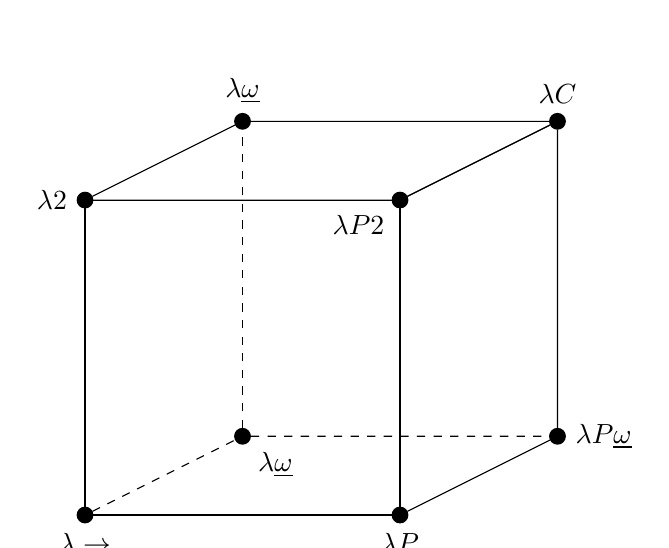
\begin{tikzpicture}
    \foreach \n/\x/\l/\p in{
    1/{( 0  , 0)}/{$\lambda \to$}/below,
    2/{( 4, 0)}/{$\lambda P$}/below,
    3/{( 2, 1)}/{$\lambda \underline{\omega}$}/south east,
    4/{( 6, 1)}/{$\lambda P \underline{\omega}$}/right,
    5/{( 0, 4)}/{$\lambda 2$}/left,
    6/{( 4, 4)}/{$\lambda P 2$}/south west,
    7/{( 2, 5)}/{$\lambda\underline{\omega}$}/above,
    8/{( 6, 5)}/{$\lambda C$}/above
    }
    {
            \node[inner sep=2pt,circle,draw,fill,label={\p:\l}] (\n) at \x {};
        }
    \draw (1) -- (2) -- (6) -- (5) -- (1);
    \draw (5) -- (6) -- (8) -- (7) -- (5);
    \draw (2) -- (4) -- (8) -- (6) -- (2);
    \draw[dashed] (1) -- (3) -- (4);
    \draw[dashed] (3) -- (7);
\end{tikzpicture}
\caption{The $\lambda$-cube or Barendregt cube}
\end{figure}

The result investigations on~\cite{barendregt} is that all the eight systems can be described with only one set of derivations rules

\begin{table}[ht]
    \centering
    \begin{tabular}{| l |} 
    \hline
    \\
    \textit{(sort)}\quad\AxiomC{$\emptyset \deriv * : \square$}
    \DisplayProof
    \\
    \\  
    \AxiomC{$\Gamma \deriv A : s$}
    \LeftLabel{\textit{(var)}\quad}
    \RightLabel{\quad if $x \notin \Gamma$}
    \UnaryInfC{$\Gamma, x : A \deriv x : A$}
    \DisplayProof
    \\
    \\
    \AxiomC{$\Gamma \deriv A : B$}
    \AxiomC{$\Gamma \deriv C : s$}
    \LeftLabel{\textit{(weak)}\quad}
    \RightLabel{\quad if $x \notin \Gamma$}
    \BinaryInfC{$\Gamma, x : C \deriv A : B$}
    \DisplayProof
    \\
    \\
    \AxiomC{$\Gamma \deriv A : s_1$}
    \AxiomC{$\Gamma, x : A \deriv B : s_2$}
    \LeftLabel{\textit{(form)}\quad}
    \BinaryInfC{$\Gamma \deriv \Pi x : A . B : s_2$}
    \DisplayProof
    \\
    \\
    \AxiomC{$\Gamma \deriv M : \Pi x : A . B$}
    \AxiomC{$\Gamma \deriv N : A$}
    \LeftLabel{\textit{(appl)}\quad}
    \BinaryInfC{$\Gamma \deriv MN : B[x := N]$}
    \DisplayProof
    \\
    \\
    \AxiomC{$\Gamma, x : A \deriv M : B$}
    \AxiomC{$\Gamma \deriv \Pi x : A . B : s$}
    \LeftLabel{\textit{(abst)}\quad}
    \BinaryInfC{$\Gamma \deriv \lambda x : A . M : \Pi x : A. B$}
    \DisplayProof
    \\
    \\
    \AxiomC{$\Gamma \deriv A : B$}
    \AxiomC{$\Gamma \deriv B' : s$}
    \LeftLabel{\textit{(conv)}\quad}
    \RightLabel{\quad if $B =_\beta B'$}
    \BinaryInfC{$\Gamma \deriv A : B'$}
    \DisplayProof
    \\
    \\
    \hline
   \end{tabular}
   \caption{Derivation rules for the systems of $\lambda$-cube}
\end{table}

\newpage
\subsection{Properties of \texorpdfstring{$\lambda C$}{}}

\begin{definition}[Expressions of $\lambda C$, $\mathcal{E}$]
    The set of $\mathcal{E}$ of $\lambda C$ is defined by:
\end{definition}
$\mathcal{E} = V \mid \square \mid * \mid (\mathcal{E}\mathcal{E}) \mid (\lambda V: \mathcal{E}. \mathcal{E}) \mid (\Pi V : \mathcal{E}. \mathcal{E})$

\begin{lemma}[Free Variable Lemma]
\end{lemma}
If $\Gamma \deriv A : B$, then $FV(A), FV(B) \subseteq \mathtt{dom}(\Gamma)$

\begin{definition}[Well-formed context]
\end{definition}
A context $\Gamma$ is well-formed if there are $A$ and $B$ such that $\Gamma \deriv A : B$

\begin{lemma}[Thinning, Permutation and Condesing Lemma]
\end{lemma}
\begin{enumerate}
    \item \textit{(Thinning)}: Let $\Gamma'$ and $\Gamma''$ be contexts such that $\Gamma' \subseteq \Gamma''$. If $\Gamma' \deriv A : B$ and $\Gamma''$ is well-formed, then also $\Gamma'' \deriv A : B$.
    \item \textit{(Permutation)}: Let $\Gamma'$ and $\Gamma''$ be contexts such that $\Gamma''$ is a Permutation of  $\Gamma'$. If $\Gamma' \deriv A : B$ and $\Gamma''$ is well-formed, then also $\Gamma'' \deriv A : B$.
    \item \textit{(Condensing)}: If $\Gamma', x : A, \Gamma'' \deriv B : C$ and $x$ does not occur in $\Gamma'', B \text{ or } C$ , then also $\Gamma, \Gamma'' \deriv B : C$.
\end{enumerate}

\begin{lemma}[Generation Lemma]
\end{lemma}
\begin{enumerate}
    \item If $\Gamma \deriv x : C$, there exists a sort $s$ and an expression $B$ such that $B =_\beta C, \Gamma \deriv B : s$ and $x : B \in \Gamma$.
    \item If $\Gamma \deriv MN: C$, then $M$ has a $\Pi$-type, i.e. there exists an expression $A$ and $B$ such that $\Gamma \deriv M : \Pi x : A. B$; moreover, $N$ fits in this $\Pi$-type $\Gamma \deriv N :A$ and finally $C =_\beta B[x := N]$
    \item If $\Gamma \deriv \lambda x : A. b : C$, then there are a sort $s$ and an expression $B$ such that $C =_\beta \Pi x : A. B$ where $\Gamma \deriv \Pi x: A. B :s$ and moreover $\Gamma, x: A \deriv b:B$
    \item If $\Gamma \deriv \Pi x:A. B:C$ then there are $s_1$ and $s_2$ such that $C \equiv s_2$, and moreover $\Gamma \deriv A : s_1$ and $\Gamma, x : A \deriv B : s_2$
\end{enumerate}

\begin{definition}
    An expression $M$ in $\lambda C$ is legal if there exists $\Gamma$ and $N$ such that $\Gamma \deriv M : N$ or $\Gamma \deriv N : M$ (typeable or inhabited)
\end{definition}

\begin{lemma}[Subexpression lemma]
    If $M$ is legal, then every subexpression of $M$ is also legal.
\end{lemma}

\begin{lemma}[Uniqueness of Types up to Conversion]
    If $\Gamma \deriv A : B_1$ and $\Gamma \deriv A : B_2$, then $B_1 =_\beta B_2$
\end{lemma}

\begin{lemma}[Substitution Lemma]
\end{lemma}
Let $\Gamma', x : A, \Gamma'' \deriv B : C$ and $\Gamma' \deriv D : A$.

Then $\Gamma', \Gamma''[x := D] \deriv B[x := D] : C[x := D]$

\begin{theorem}[Church-Rosser Theorem; CR; Confluence]
    The Church-Rosser property holds for $\lambda C$.
\end{theorem}

\begin{theorem}[Strong Normalization Theorem or Termination Theorem]
    Every legal $M$ is strongly normalizing.
\end{theorem}

\begin{theorem}[Decidability of Well-typedness and Type Checking]
    In $\lambda C$ and its subsystems, the questions of Well-typedness and Type Checking are decidable.
\end{theorem}

The question of \textit{Term finding} it is decidable for $\lambda \to$ and $\lambda \underline{\omega}$, but undecidable for the rest.
All the proofs can be found on~\cite{barendregt}.

\subsection{Exercises}
\subsubsection{6.6}
Given $M \equiv \lambda S : *. \lambda P : S \to *. \lambda x : S. (P x \to \perp)$.

\begin{exercise}[(a)]
    Which is the smallest system in the $\lambda$-cube in which $M$ may occur?
\end{exercise}
The smallest is $\lambda C$. Taking the eight possibilities
\begin{itemize}
    \item $\perp$ needs $(\square, *)$
    \item $\lambda x : S. (P x \to \perp)$ needs $(*, \square)$
    \item $\lambda P : S \to *. \lambda x : S. (P x \to \perp)$ needs $(\square, \square)$
\end{itemize}

\begin{exercise}[(b)]
    Proof $M$ is legal
\end{exercise}
\begin{flagderiv}
    \assume{}{S : *}{}
    \assume{}{P : S \to *}{}
    \assume{}{x : S}{}
    \step{}{Px : S}{}
    \step{}{\perp : *}{}
    \step{}{Px \to \perp : *}{}
    \conclude{}{\lambda x : S. (P x \to \perp) : S \to *}{}
    \conclude{}{\lambda P : S \to *. \lambda x : S. (P x \to \perp) : (S \to *) \to S \to *}{}
    \conclude{}{\lambda S : *. \lambda P : S \to *. \lambda x : S. (P x \to \perp) : S \to (S \to *) \to S \to *}{}
\end{flagderiv}

\begin{exercise}[(c)]
    How could you interpret $M$ if $A \to \perp$ encodes $\neg A$?
\end{exercise}
It is a function that maps $S$ and $P$ to $\overline{P}$, something that is true if $P$ does not hold, therefore it is impossible.

\newpage
\bibliographystyle{alpha}
\bibliography{report}

\end{document}
